\documentclass[fleqn]{jbook}
\usepackage{physpub}

\begin{document}

\begin{question}{専攻 問題6}{}
図1は、レーザー干渉計を用いて、重力加速度を測定するための概念図で
ある。反射鏡$M_d$、$M_f$はコーナーリフレクターと呼ばれるもので、図
2に示すように平面鏡を3枚互いに直交させたものである。$M_f$は実験室系に固定し、$M_d$をある位置から自由に落下させる。これに関する以下の設問に答えよ。

\begin{subquestions}
\SubQuestion
コーナリフレクターに図2のように入射する光ビームは、入射方向と平行に戻る。これを示せ。

\SubQuestion
自由落下中は、光検出器からは、図3のように変化する信号が得られる。
変化する信号が中央線を切る時間を図3のように$t_1$、$t_2$、$t_3$と
するとき、光の波長を$\lambda$として、時刻$t_2$における平均の重力加速度を求めよ。

\begin{center}
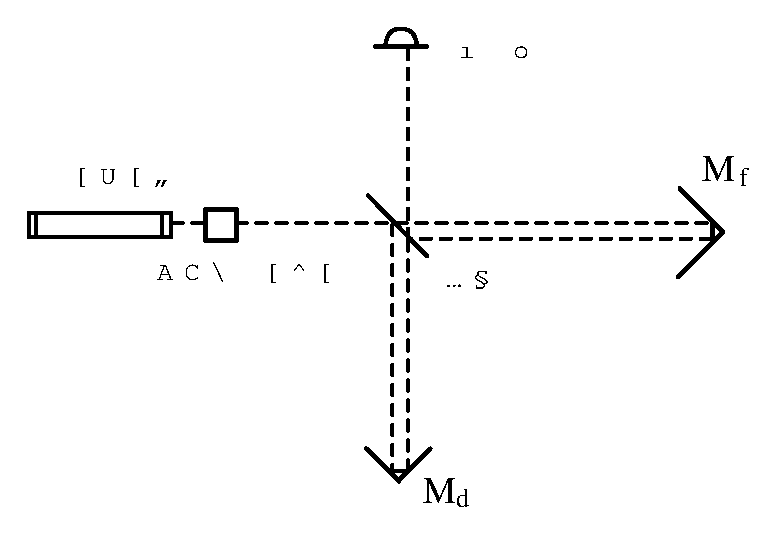
\includegraphics[clip,height=40mm,width=45mm]{1997phy6-1.eps}
\includegraphics[clip,height=35mm,width=35mm]{1997phy6-2.eps}
\includegraphics[clip,height=40mm,width=40mm]{1997phy6-3.eps}
\end{center}

\SubQuestion
重力加速度の相対測定精度を10$^{-9}$としたい。$M_d$に向かうレーザービームが理想的な平面波と仮定できる場合、ビーム光と鉛直線とのずれ角は、いくら以内でなければならないか。

\SubQuestion
空気抵抗は大きい誤差になるので、$M_d$(質量 100g、断面積 10 cm$^2$)は真空中を落下させなければならない。落下速度が3m/sの時、残留ガスによる加速度が重力加速度より9桁小さくなるために必要な真空度を求めよ(必要な真空度は1mPa以下であり、アボガドロ数は6$\times$ 10$^{23}$、1気圧は10$^5$Pa、1モルの気体は室温・1気圧で 20 {\it{l}}の体積を占め、残留ガスの分子量を30とする)。

\SubQuestion
$M_d$はアースされた金属の菅の中を落下する。$M_d$が電荷を帯びている
と、$M_d$の落下加速度にどのような影響が生じるか。

\end{subquestions}
\end{question}
\begin{answer}{専攻 問題6}{}
\begin{subanswers}
%
\SubAnswer

\parbox[t]{110mm}{右の図の3枚の平面鏡の法線方向を、それぞれ$x,y,z$軸
にとる。入射光の方向ベクトルを$(a,b,c )$とする。すると方向ベクトルは、
yz平面で反射して$(-a,b,c)$、xy平面で反射して$(-a,b,-c)$、zx平面で反射
して$(-a,-b,-c)$、の様に変わるので、入射光と平行に反射する。}\parbox[t]{10mm}
{\vspace*{-5mm}
\begin{center}
\includegraphics[clip,height=45mm,width=45mm]{1997phy6-4.eps}
\end{center}
}

\SubAnswer

\parbox[t]{50mm}{\vspace*{-15mm}
\begin{center}
\includegraphics[clip,height=45mm,width=45mm]{1997phy6-5.eps}
\end{center}}\parbox[t]{110mm}{
問題図中の $t_1,t_2,t_3$は、左図のそれぞれ$\times$がふってあるところで
ある。$t_1 \sim t_2$間にコーナーリフレクターは、半波長分落下している。
また、同様に$t_2 \sim t_3$間にコーナーリフレクターは、半波長分落下して
いる。

よって、$t=0$におけるコーナーリフレクターの落下速度を$v_0$とおくと、以下の関係式が得られる。
(重力加速度を$g$、入射光の波長を$\lambda$とおいた)
\[\left\{
  \begin{array}{l}
    (\frac{1}{2} g{t_2}^2+v_0t_2)-(\frac{1}{2} g{t_1}^2+v_0t_1)= \frac{\lambda}{
2} \\
    (\frac{1}{2} g{t_3}^2+v_0t_3)-(\frac{1}{2} g{t_2}^2+v_0t_2)= \frac{\lambda}{
2}
  \end{array}
\right. \]
}

両者から$v_0$を消去して整理すると

\[\underline{g = \lambda \cdot \frac{2t_2-(t_1+t_3)}{(t_3-t_2)(t_3-t_1)(t_2-t_1)
}}\]
%
\SubAnswer

\parbox[t]{100mm}{ビームが鉛直線と角$\varphi$をなしているとする。
この時、 $M_d$ で反射する光路の変化 $\Delta l^{\prime}$ は、実際に $M_d$ が動い
た $\Delta l$と
\[\Delta l = \Delta l^{'} \cos \varphi\]

の関係がある。ここで前問と同様に $g$ を求めてやると
\[ g(\varphi) = \lambda \cdot \frac{2t_2-(t_1+t_3)}{(t_3-t_2)(t_3-t_1)(t_2-t_1)} 
\cos \varphi \]
となり、$\cos \varphi$の項がつく。従って、正しい $(\varphi = 0)$ものに比べ
\[
\frac{g(0)-g(\varphi)}{g(0)} =  1-\cos \varphi \simeq \frac{\varphi ^2}{2} 
\]
(∵ $\varphi \simeq 0$ の時 $\cos \varphi = 1 - \frac{\varphi ^2}{2}$)
}\parbox[t]{60mm}{
\begin{center}
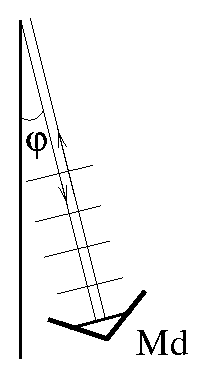
\includegraphics[clip,height=40mm,width=20mm]{1997phy6-6-1.eps}
\hspace{5mm}
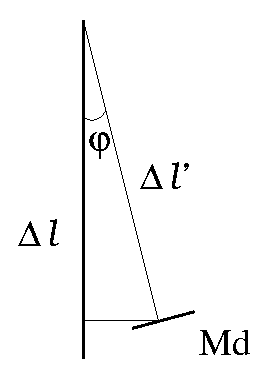
\includegraphics[clip,height=40mm,width=26mm]{1997phy6-6-2.eps}
\end{center}
}

の差がある。これは相対測定精度とみなせるので、それが$10^{-9}$ となるためには$\frac{\varphi ^2}{2} = 10 ^{-9}$となればよい。 よって、
\[ \varphi = \sqrt{\mathstrut 2 \times 10^{-9}} = 4,5 \times 10^{-5} \quad {\Unit{[{\Unit{rad}}]}} \]

従って、ずれ角は \underline{$4.5 \times 10^{-5}[{\Unit{rad}}]$}以下でなくてはならないこと
がわかる。

%
\SubAnswer

まず、室温での残留ガスの二乗平均速度を求める。
\[ \frac{1}{2} m\bar{{v}^2} = \frac{3}{2} kT = \frac{3}{2} \frac{R}{N_A} T \]
\[ \mbox{∴} \quad \bar{{v}^2} = \frac{3RT}{N_A m} \]

ここで $pV = nRT$ と、与えられた条件より
\[RT = 20 [\Unit{atm} \cdot l {\Unit{ / mol}}] = 2 \times 10^3 [{\Unit{Pa \cdot m^3 / mol}} ]\]

また、$N_A m = 3 \times 10^{-2} [{\Unit{kg}/ \Unit{mol}}]$ より
\[\bar{{v}^2} = 2 \times 10^{5} [{\Unit{m^2 / s^2}}]\]

したがってこの時
\[\bar{{v_x}^2} = \frac{2}{3} \times 10^5 \hspace{10mm} \Yueni \sqrt{\bar{{v_x}^2}} = 258.2[{\Unit{m/s}}]\]

$M_d$に対し、下から衝突する残留ガス分子は、本来よりも $3[{\Unit{m/s}}]$ だけ速く、
上から衝突するものは $3[{\Unit{m/s}}]$ だけ遅く感じることになるので、
\begin{eqnarray}
\bar{{v_{down}}^2} & = 3(\sqrt{\mathstrut \bar{{v_x}^2}}+3)^2  & = 2.0467 \times 10^5 [{\Unit{m^2/s^2}}] \nonumber \\
\bar{{v_{up}}^2} & = 3(\sqrt{\mathstrut \bar{{v_x}^2}}-3)^2  & = 1.9538 \times 10^
5 [{\Unit{m^2/s^2}}] \nonumber
\end{eqnarray}

\parbox[t]{100mm}{
$M_d$ の運動について
\[Ma = Mg - (p_{up} -p_{down})S\]

問題の条件を満たすためには、
\[\frac{(p_{up} -p_{down})S}{Mg} < 10^{-9}\]
\[p_{up} -p_{down} < 10^{-9} \cdot \frac{0.1 \times 10}{1.0 \times 10^{-3}} = 10^{-6}\Unit{Pa}\]

ここで、
\[p = \frac{N}{N_A} \frac{RT}{V} = \frac{Nm}{3V} \bar{v^2}\]
}\parbox[t]{60mm}{\vspace*{-5mm}
\begin{center}
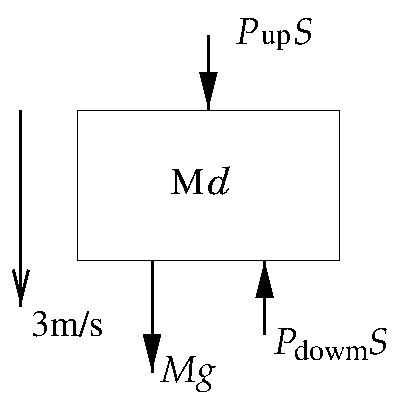
\includegraphics[clip,height=50mm,width=50mm]{1997phy6-7.eps}
\end{center}
}

よって、必要な条件は結局
\[\frac{Nm}{3V} < 10^{-10}\]

ここで、1気圧のとき
\[10^5 = \frac{Nm}{3V} \times 2 \times 10^5 \hspace{10mm} ∴ \quad \frac{Nm}{3V} = 5 \times 10^{-1}\]

したがって、必要な真空度は$2 \times 10^{-10} [{\Unit{atom}}] = \underline{2 \times 10^{-5}
 [{\Unit{Pa}}]}$
%
\SubAnswer

周りはアースされた金属管であるから、$M_d$ に電荷があると、その内部表面に $M_d$ 
と反対の電荷が
誘起され、いわゆる遮蔽効果が観察される。$M_d$が静止していれば、誘起される電荷は
ポテンシャルが
最低となる分布をしておわるが、$M_d$が動くとこの分布も常に変化し、新たにポテンシ
ャルが最低と
なるような分布を作ろうとする。この時、移動する電子は金属内で抵抗を受け、ジュール
熱を発する。
このエネルギーは$M_d$の持つエネルギーの減少分で補われねばならないので、結果とし
て$M_d$の運動
エネルギーは減り、減速される。

(誘導される電荷が、$M_d$が動くのを妨げる方向に力を及ぼす、という書き方もある)

\end{subanswers}
\end{answer}


\end{document}
